\documentclass{ximera}
%%%
\title{TikZ Craziness}
\author{Robert Kelvey, robertkelvey@gmail.com}

\usepackage{multicol}
\usepackage{graphicx}
\usepackage{gnuplottex}
\usepackage[latin1]{inputenc}
\usepackage{tikz}
\usepackage{pgfplots}

\begin{document}

\begin{abstract}
    In this activity, we try out something crazy in tikZ. Precisly, we are trying to place an answer box inside of a tikZ node.
\end{abstract}

\maketitle

\begin{question}
Enter the secret answer!

\begin{center}
    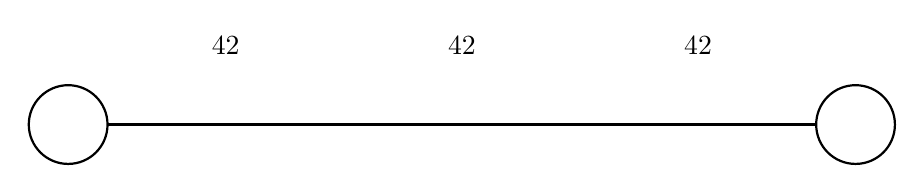
\begin{tikzpicture}
        \draw[thick] (0,0) circle (0.5); 
        \draw[thick] (0.5,0) -- (9.5,0);
        \draw[thick] (10,0) circle (0.5);
        \node at (2,1) {$\answer{42}$};
        \node at (5,1) {$\answer{42}$};
        \node at (8,1) {$\answer{42}$};
    \end{tikzpicture}
    
\end{center}


\end{question}

LESSON: That did not work...And we know that it will never work. Tikz turns its drawn output into a .svg image, so there is no hope of obtaining an answer box in the final html output. 






\end{document}
